\documentclass[12pt]{article}
\usepackage[a4paper,top=1pt,bottom=2pt,left=1pt,right=1pt,marginparwidth=1pt,headheight=1pt]{geometry}

% Encoding Settings
\usepackage[T1]{fontenc}
\usepackage[utf8]{inputenc}



% Font Settings
\usepackage{times}

% Define a new font called Tinyb. This font can maintain its shape even in very small fontsize:
% \usepackage{lmodern}
% \rmfamily
% \DeclareFontShape{T1}{lmr}{bx}{sc}{<-> cmr10}{}% USE BOLD SCSHAPE NOT OTHERWISE DEFINED
% %%% MATH FONT FIX
% \DeclareFontFamily{OML}{zlmm}{}
% \DeclareFontShape{OML}{zlmm}{m}{it}{<-> lmmi10}{}
% \DeclareFontShape{OML}{zlmm}{b}{it}{<->ssub * zlmm/m/it}{}
% \DeclareFontShape{OML}{zlmm}{bx}{it}{<->ssub * zlmm/m/it}{}
% \DeclareMathVersion{Tinyb}
% \SetSymbolFont{operators}{Tinyb}{T1}{lmr}{bx}{sc}
% \SetSymbolFont{letters}{Tinyb}{OML}{zlmm}{m}{it}
% \newenvironment{tinyb}{\bgroup\tiny\bfseries\scshape\mathversion{Tinyb}}{\egroup}



% Paragraph Settings
\usepackage{setspace}
\onehalfspacing
\usepackage{parskip}
\setlength{\parindent}{0in}



% Reference Settings
\usepackage[
    backend=biber,
    style=ieee,
]{biblatex}
\addbibresource{References.bib}

% Elegantly break long doi field
% \setcounter{biburllcpenalty}{100}
% \setcounter{biburlucpenalty}{100}
% \setcounter{biburlnumpenalty}{100}



% Figure Settings
\usepackage{graphicx} % Required for inserting images
\renewcommand{\figurename}{\textbf{Fig.}}

\usepackage{float}

% Enable two figures in one line:
% \usepackage{subfig}
% \begin{figure}[htbp!]
%   \centering
%   \subfloat[Before re-initialization]{\includegraphics[width=0.5\textwidth]{Figures/Before re-initialization.pdf}\label{fig:f1}}
%   \hfill
%   \subfloat[After re-initialization]{\includegraphics[width=0.5\textwidth]{Figures/After re-initialization.pdf}\label{fig:f2}}
%   \centering
%   \caption{Swarm distribution before and after reinitializing transitional particles on a one-dimensional problem}
%   \label{fig:before_and_after_reinitialization}
% \end{figure}



% Array Settings
\usepackage{array}
\newcolumntype{R}{>{$}r<{$}} % math-mode version of "r" column type
\newcolumntype{C}{>{$}c<{$}} % math-mode version of "c" column type
\newcolumntype{L}{>{$}l<{$}} % math-mode version of "l" column type

% defines a new type of column called Y based on a X column (this column type is defined by the tabularx package and it is basically a p{ <width>} column, where <width> is calculated by the package) but typesets the content using \small font size and with ragged-right text.
% \newcolumntype{Y}{>{\small\raggedright\arraybackslash}X}

% Modify the space on the bottom and top of each cell:
\usepackage{cellspace}
% \addtolength{\cellspacetoplimit}{5pt}
% \addtolength{\cellspacebottomlimit}{5pt}

\usepackage{multirow}
\usepackage{tabularx,booktabs}
\usepackage{longtable}
\usepackage{relsize}

% \renewcommand{\thetable}{S\arabic{table}}  % Rename the table names to Table Sx.

% Equally spread columns to fulfill the whole table.
% \begin{longtable}[c]{@{\extracolsep{\fill}}Lllllllll}

% Define a horizontal line that only appears in specific columns:
% \usepackage{hhline}
% \hhline{~----~~}  % Use as \hline, but the column with ~ will not have a horizontal line.



% Hyper-reference Settings
\usepackage{hyperref}
\hypersetup{
    colorlinks=true,
    linkcolor=cyan,
    citecolor=cyan,
    urlcolor=cyan,
}
% \usepackage[all]{hypcap} 
% \makeatletter
% \AtBeginDocument{\def\@citecolor{cyan}}  % Define citing 
% \AtBeginDocument{\def\@urlcolor{cyan}}
% \AtBeginDocument{\def\@linkcolor{cyan}}
% \makeatother

% Make the brackets of equation citation blue:
% \hyperref[eq:clpso_velocity]{(\ref*{eq:clpso_velocity})}



% Mathematical Settings 
\usepackage{mathtools}
\usepackage{amssymb,mathrsfs}  % Typical maths resource packages
\usepackage{amsthm}
\usepackage{amsmath}
\usepackage{nccmath}  % To narrow parskip between two equations. \useshortskip



% Equation Settings
% \counterwithout{equation}{chapter}

% To use the large bracket on one side of equation:
% \begin{equation}
%     \label{eq:sum}
%     Sum = 
%     \begin{cases}
%        Y_1 + Y_2 + Y_3, & \theta = 3 \\
%        Y_1 + Y_2 + \cdots + Y_8, & \theta = 8
%     \end{cases}
% \end{equation}



% Algorithm Settings
\usepackage{algorithmic}
% \usepackage{algpseudocodex}
\renewcommand{\algorithmicrequire}{\textbf{Input:}}
\renewcommand{\algorithmicensure}{\textbf{Output:}}



% Enumerate Settings
% \usepackage{enumitem}
% \begin{enumerate}[label={(\arabic*).}]
%     \item XXX
%     \item XXX
% \end{enumerate}


% Line Number Settings
\usepackage{lineno}
% \linenumbers  % Uncomment this line to turn on the line number settings



% Code Settings
% \usepackage{courier}
% \usepackage{minted}


% Subfile Settings
% \usepackage{subfiles}
% \providecommand{\topdir}{.}
% \addglobalbib{\topdir/References.bib}



% Attach File Settings
\usepackage{attachfile}
% \attachfile[icon=Paperclip]{Test.pdf}



% Additional Settings

% Define a checkbox:
% \newcommand{\checkbox}[1]{%
%   \ifnum#1=1
%     \makebox[0pt][l]{\raisebox{0.15ex}{\hspace{0.1em}$\checkmark$}}%
%   \fi
%   $\square$%
% }

\usepackage{blindtext}
\usepackage{multicol}
\usepackage{color}
\setlength{\columnsep}{0.2cm}
\setlength{\columnseprule}{1pt}
\def\columnseprulecolor{\color{black}}

\usepackage{xpatch}
\xpatchcmd{\NCC@ignorepar}{%
\abovedisplayskip\abovedisplayshortskip}
{%
\abovedisplayskip\abovedisplayshortskip%
\belowdisplayskip\belowdisplayshortskip}
{}{}

\setlength{\parindent}{0in}
\setlength{\parskip}{0in}

\setlength{\belowdisplayskip}{0pt} \setlength{\belowdisplayshortskip}{0pt}
\setlength{\abovedisplayskip}{0pt} \setlength{\abovedisplayshortskip}{0pt}



\usepackage{soul}
\usepackage[dvipsnames]{xcolor}
\newcommand{\bulletPoint}[1]{\ul{\textit{\textbf{#1}}}}


% For better text align
\usepackage{ragged2e}



\begin{document}
\singlespacing


\begin{multicols*}{2}

\scriptsize

\raggedright

\bulletPoint{Knowledge Representation}:

Capturing knowledge in a way suitable for computer manipulation.

– Predicate Calculus/Neural Network;   
– Graph / Tree

% \bulletPoint{Search}:

% Problem-solving techniques. systematically explores a space of problem states. 

% \bulletPoint{State Space Representation (SSR)}:

% Define possible States; Transitions between these states based on Rules: observation/actions. SSR is used to model the different configurations a system can be in; and find the possible paths to reach a solution.


\bulletPoint{Euler's Conclusion}:

Unless a graph contained either exactly 0 or 2 nodes of odd degree, a walk over a graph in the manner described by the bridges of Konigsberg problem is impossible. 

%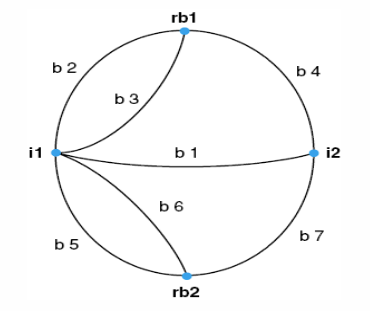
\includegraphics[scale=0.3]{euler.png}

% \bulletPoint{State Space Search}:
% A state space is represented by a four-tuple [N, A, S, GD],where:

% – N is the set of nodes or states of the graph. These correspond to the states in a problem-solving process

% – A is the set of arcs (or links) between nodes. These correspond to the steps in a problem-solving process

% – S, a nonempty subset of N, contains the start state(s) of the problem

% – GD, a nonempty subset of N, contains the goal state(s) or the problem. The states in GD are described using either:

% • a measurable property of the states visited in the search

% • a property of the path developed in the search


% \bulletPoint{Strategies for State Space Search}:

%  A state space is represented by a four-tuple [N, A, S, GD],where:

% – N is the set of nodes or states of the graph. These correspond to the states in a problem-solving process

% – A is the set of arcs (or links) between nodes. These correspond to the steps in a problem-solving process

% – S, a nonempty subset of N, contains the start state(s) of the problem

% – GD, a nonempty subset of N, contains the goal state(s) or the problem. The states in GD are described using either:

% • a measurable property of the states visited in the search

% • a property of the path developed in the search

\bulletPoint{Graph Terminologies}:

– Node/Arch/Path/Tree;  
– Directed/Rooted Graphs;  
– Parent, Siblings/Ancestor/Descendant

\bulletPoint{State Space Approach Examples}:

– Tic-Tac-Toe/8-puzzle;  
– TSP: The number of possible ways to visit N cities, (N-1)!

%\bulletPoint{Data-driven and Goal-driven}:

%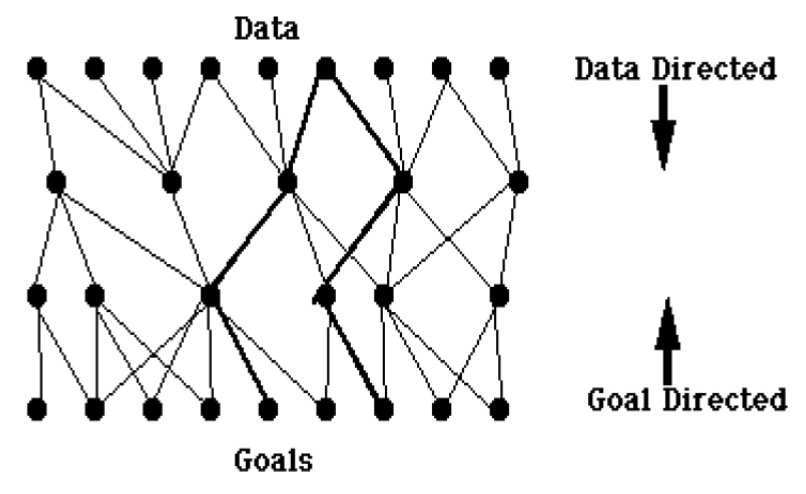
\includegraphics[scale=0.15]{data_goal.png}

\bulletPoint{Backtracking}:

– Depth-first search for CSPs;  
– Basic uninformed search for CSPs

Notations:

– CS = Current State (the state currently under consideration)

– SL = State List (the list of states in the current path being pursued. If a
goal is found, SL contains the ordered list of states on the solution path)

– NSL = New State List (the list of new states contains nodes awaiting
evaluation, i.e., nodes whose descendants have not yet been generated
and searched) (Unprocessed states)

– DE = Dead Ends (the list of states whose descendants have failed to
contain a goal node. If these states are encountered again, they will be
deleted as elements of DE and eliminated)

– CS (Current State) is always equal to the state most recently added to SL
and represents the "frontier" of the solution path currently being explored.

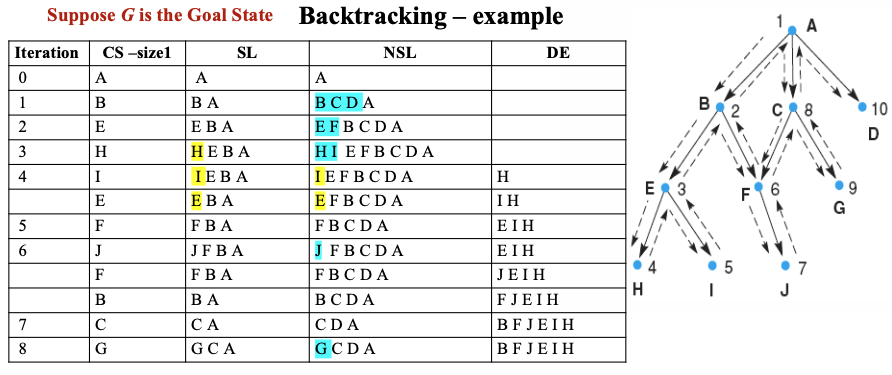
\includegraphics[scale=0.31]{images/Backtracking.png}

\bulletPoint{Breadth-first}:

– open - states that have been generated but whose children have not been examined. Right in, left out; first-in-first-out. (FIFO)

– closed - states that have already been examined. Add from the left. 

– Memory used: $B ^ n$

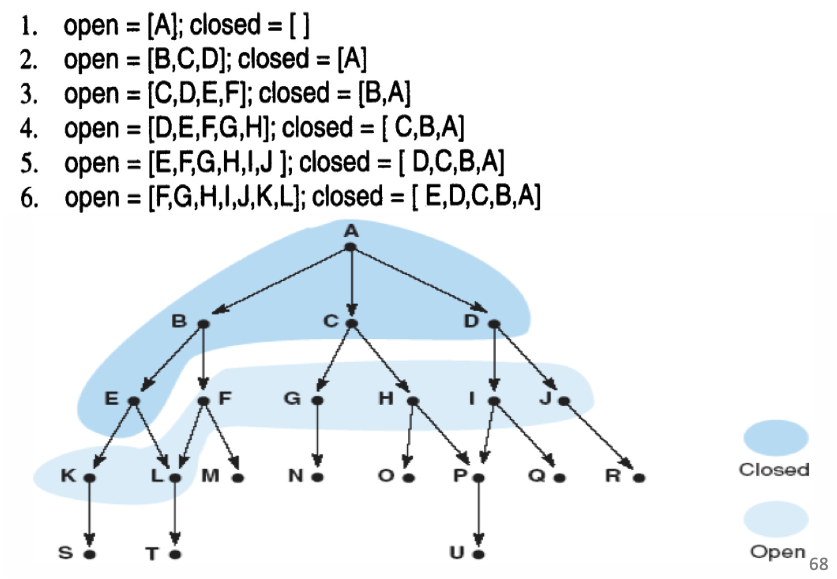
\includegraphics[scale=0.3]{images/breadth-first.png}

\bulletPoint{Depth-first}:

–  open is maintained as a stack, or last-in-first- out (LIFO) structure. Open is similar to NSL in backtrack

– closed‐ states that have already been examined. An union of DE and SL in backtrack

– Memory used: $B * n$

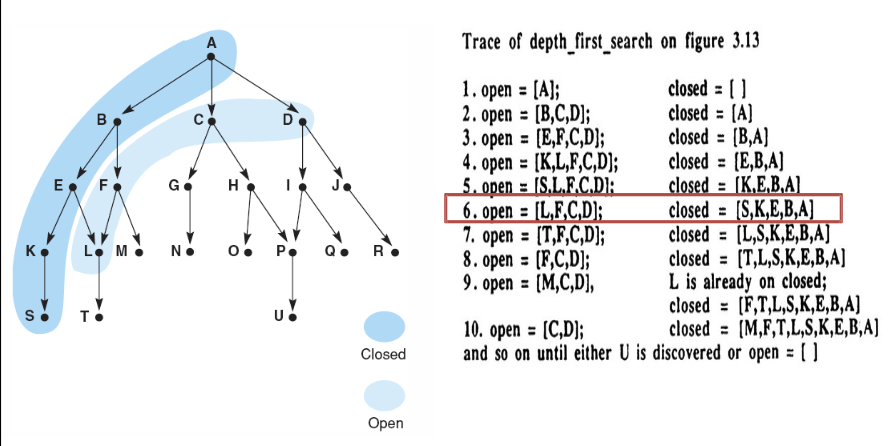
\includegraphics[scale=0.3]{images/depth-first.png}

\bulletPoint{Depth-First with Iterative Deepening}:

Depth bound from 1, and increase by one each time.


\bulletPoint{Uninformed}: 

BFS: $b^d$, $b^d$;    DFS: $b^m$, $b*m$;     IDS: $b^d$, $b*d.

b- maximum branching factor of the search tree; d- depth of the least-cost solution; m- maximum depth of the state space (may be unlimited )

\bulletPoint{Informed}: 
Hill-Climbing, Best-First(Greedy), A*

\bulletPoint{Heuristic Search}:

–  Hill-Climbing

–  Best-First-Search: 

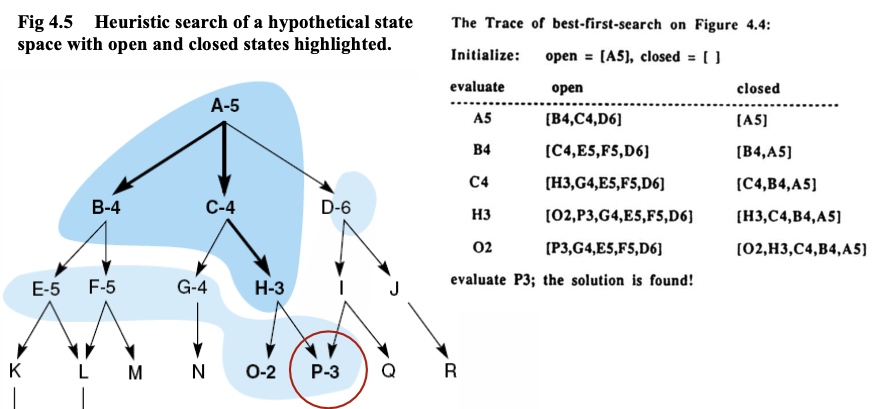
\includegraphics[scale=0.3]{images/BFS.png}

- Evaluation function f(n)=g(n)+h(n):  

g(n) = cost so far to reach n;  
h(n) = estimated cost to goal from n;  
f(n) = estimated total cost of path through n to goal. 

– When g(n)=0, Greedy Best-First;  
–  A* search is optimal, when h(n) is admissible. h(n) is always under-estimated/same as the actual cost from n to a goal.

\bulletPoint{Minimax}:

–  ALPHA-BETA pruning: Directly prune the whole right node. 

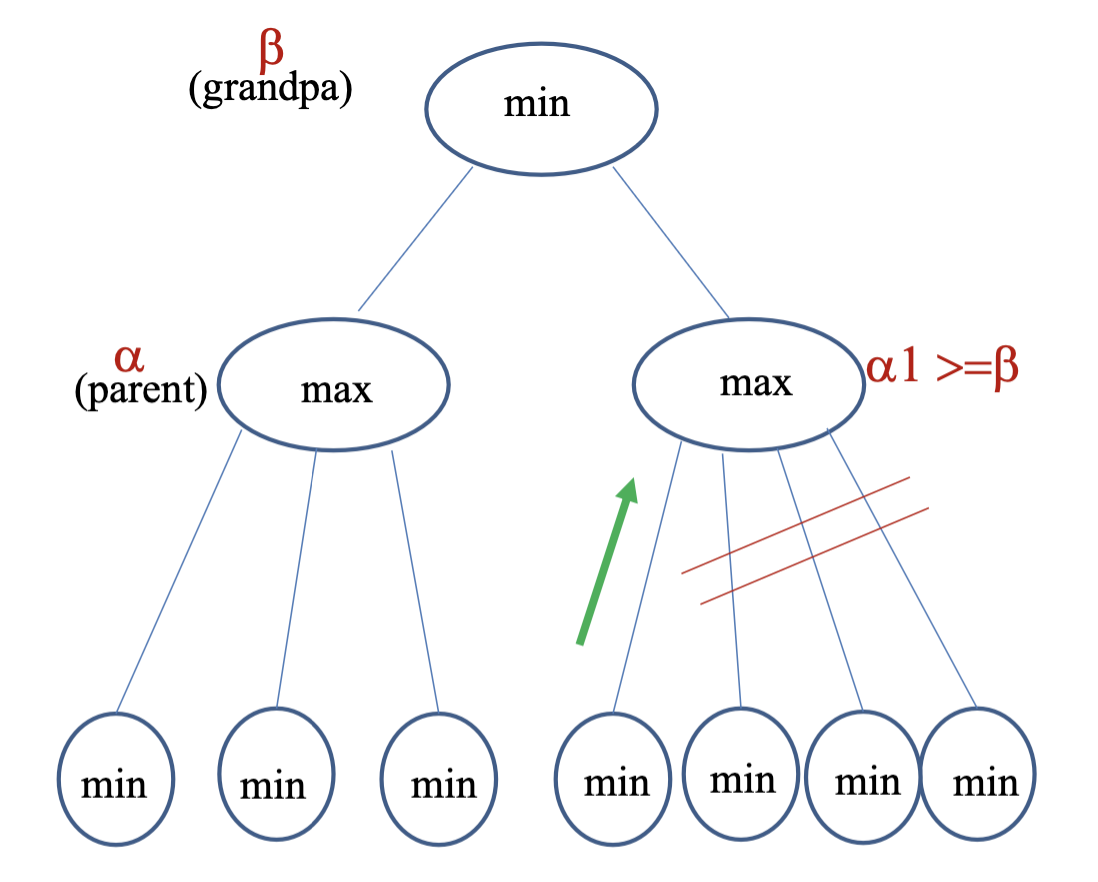
\includegraphics[scale=0.17]{images/alpha-beta.png}
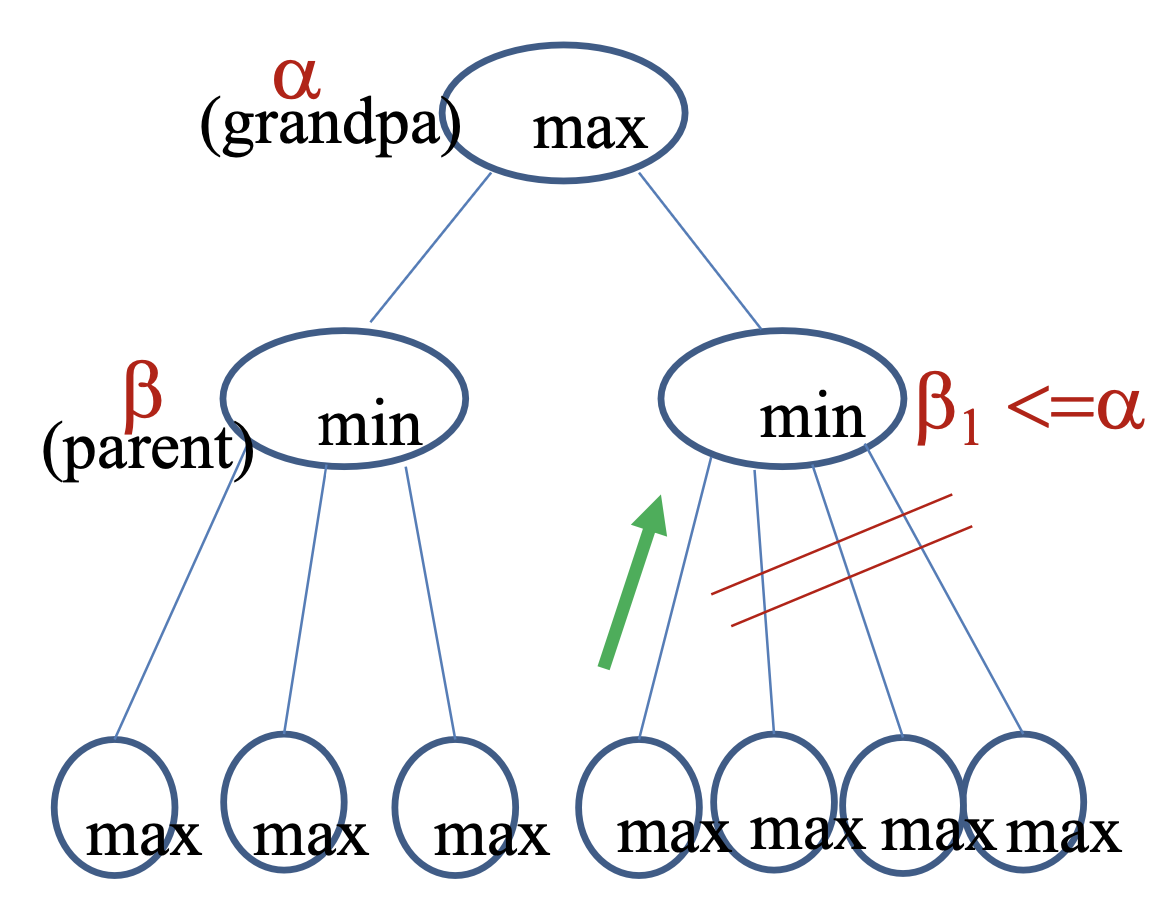
\includegraphics[scale=0.16]{images/beta-alpha.png}

\bulletPoint{Association rule}:

An \textit{association rule} is an implication of the form \( X \rightarrow Y \), where \( X \subseteq I \), \( Y \subseteq I \), and \( X \cap Y = \emptyset \), e.g., \(\{ \text{Diaper, Milk} \} \rightarrow \{ \text{Beer} \}\),
$\text{Support}(X) = \frac{\sigma(X)}{|T|} = P(X) \quad \textit{Support of itemset } X: \textit{the Probability of } X$
$\text{Support}(X \rightarrow Y) = \frac{\sigma(X \cup Y)}{|T|} = P(X \cup Y)$
$\text{Confidence}(X \rightarrow Y) = \frac{\sigma(X \cup Y)}{\sigma(X)} = \frac{P(X \cup Y)}{P(X)} = P(Y \mid X)$
There are a total of $3^d - 2^{d + 1} + 1$ possible rules for a dataset 
containing $d$ items. $2^{d}-1$  item sets. 

\bulletPoint{The Apriori Principle}:

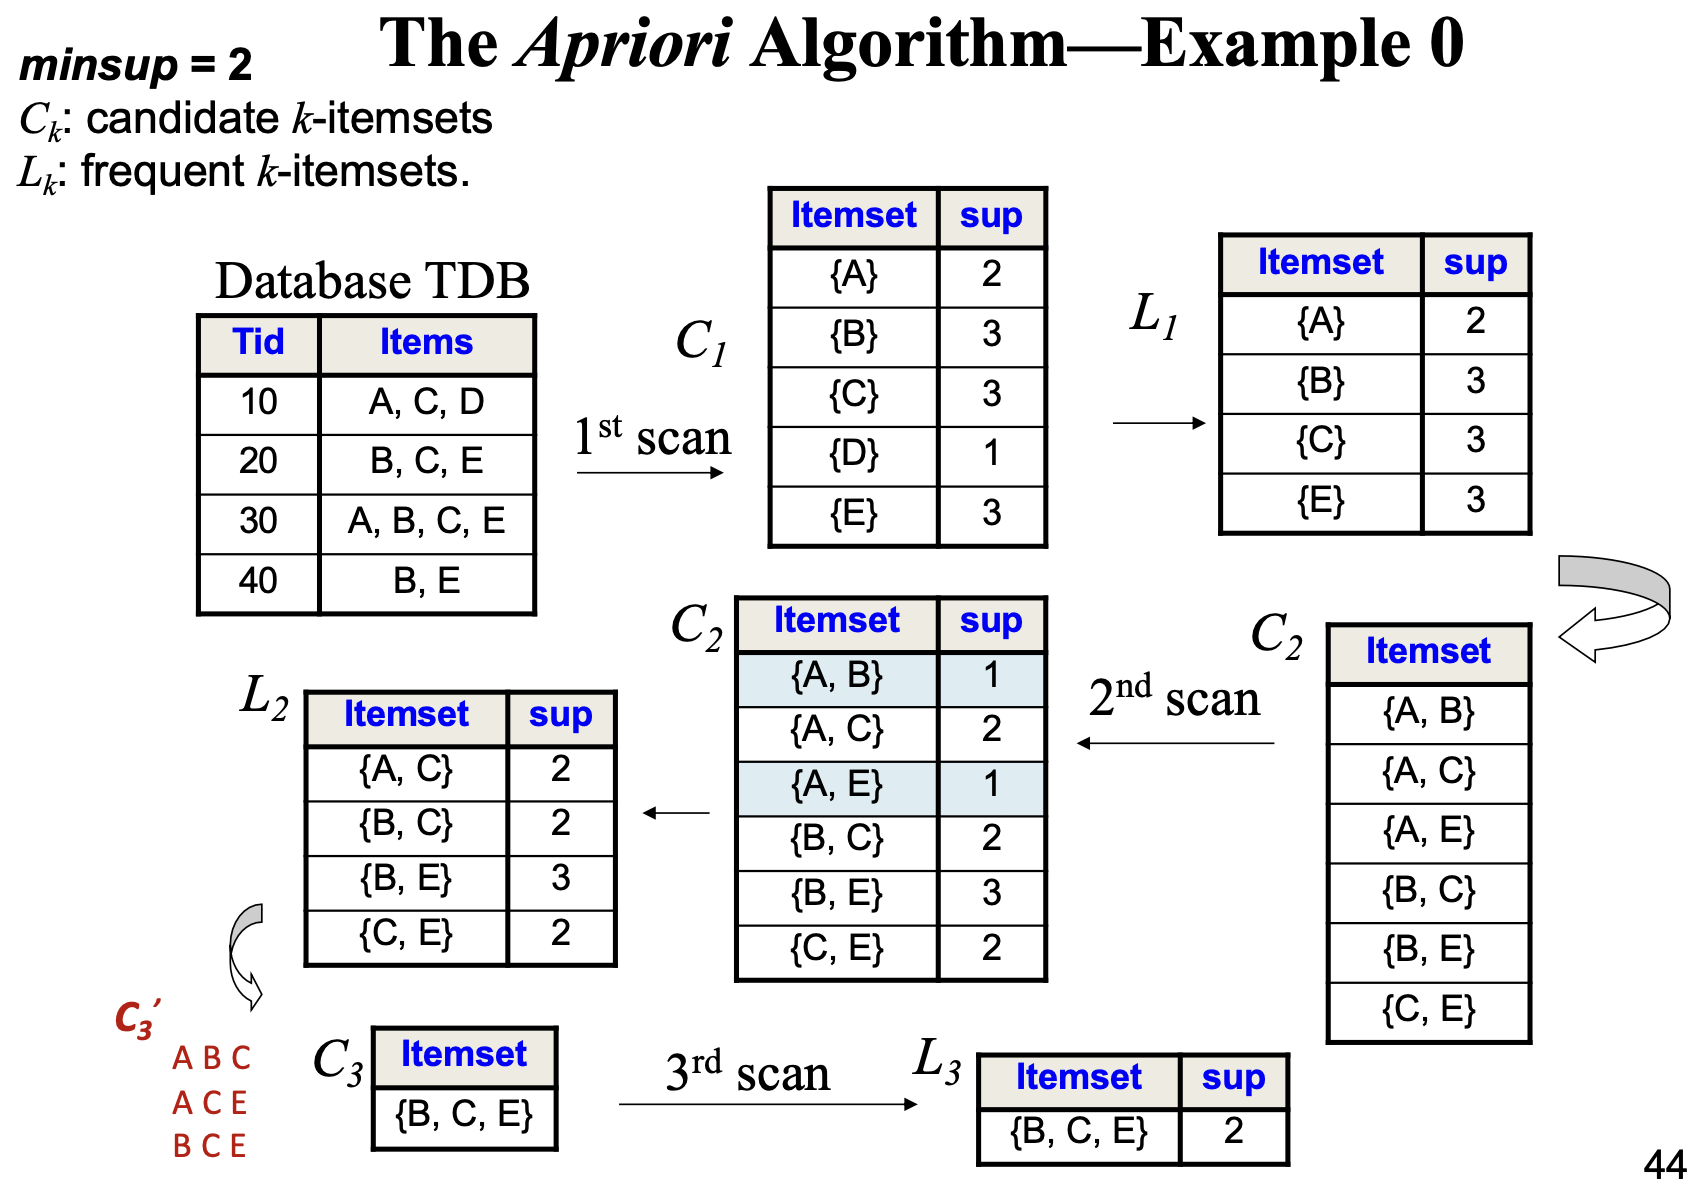
\includegraphics[scale=0.3]{images/Apriori.png}

\bulletPoint{The FP-Growth Algorithm}:

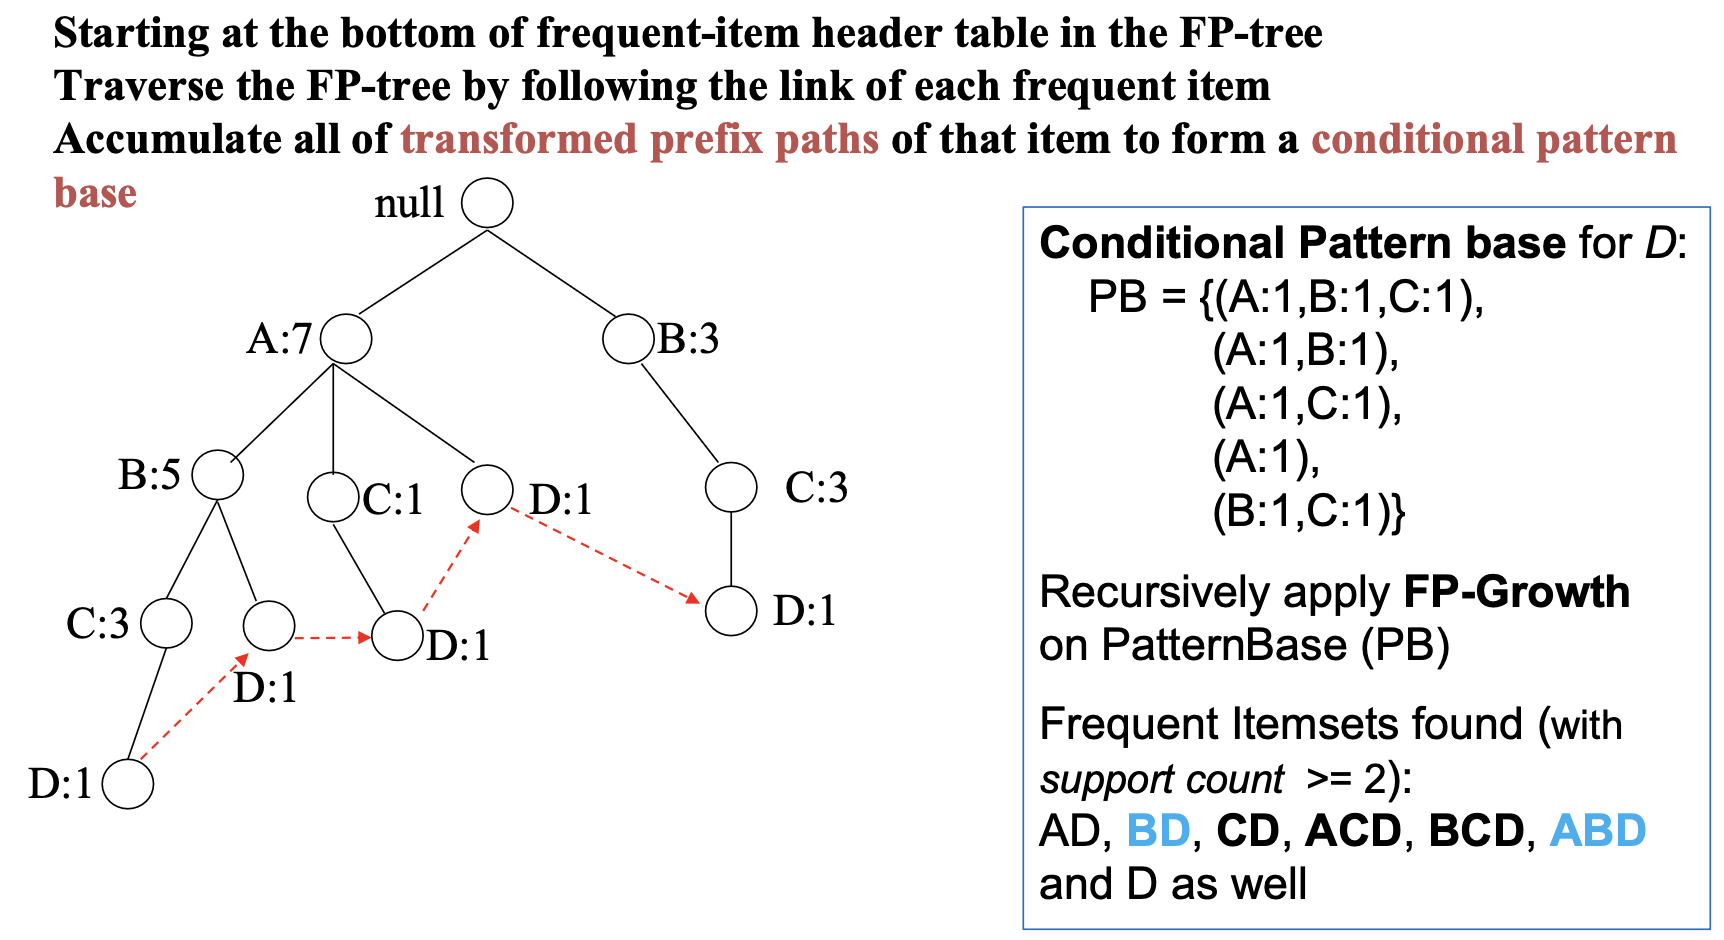
\includegraphics[scale=0.3]{images/FP-Growth.png}

\bulletPoint{Association Rule Generation}:

if  \(\frac{\sigma(Y)}{\sigma(X)} \geq \textit{minconf}\):
$X\subset Y$,  \( X \rightarrow Y -X\).  If \( |Y| = k \), then there are \( 2^k - 2 \) candidate association rules (ignoring: \( Y \rightarrow \emptyset \) and \( \emptyset \rightarrow Y \)).  

Lift is a simple correlation measure between two item sets \(X\) and \(Y\), defined as

$\text{Lift}(X, Y) = \frac{\text{Confidence}(X \rightarrow Y)}{\text{Support}(Y)} = \frac{P(X \cup Y)}{P(X)P(Y)} = \frac{P(Y \mid X)}{P(Y)}$

where
$\text{Lift}(X, Y) =
\begin{cases} 
1, & \text{if } X \text{ and } Y \text{ are independent;} \\
>1, & \text{if } X \text{ and } Y \text{ are positively correlated;} \\
<1, & \text{if } X \text{ and } Y \text{ are negatively correlated.}
\end{cases}$

\bulletPoint{Information Gain}:

The amount of information in \( D \) with \( m \) distinct classes can be defined as:

$\text{Info}(D) = - \sum_{i=1}^{m} p_i \log_2(p_i)$

If attribute \(A\) is used to split \(D\) into \(v\) subsets, \(\{D_1, D_2, \ldots, D_v\}\), the resulting information is

$\text{Info}_A(D) = \sum_{j=1}^{v} \frac{|D_j|}{|D|} \times \text{Info}(D_j)$

Information gain is defined as the difference between the original information (before splitting) and the remaining information (after splitting \(D\) by \(A\)):

$\text{Gain}(A) = \text{Info}(D) - \text{Info}_A(D)$

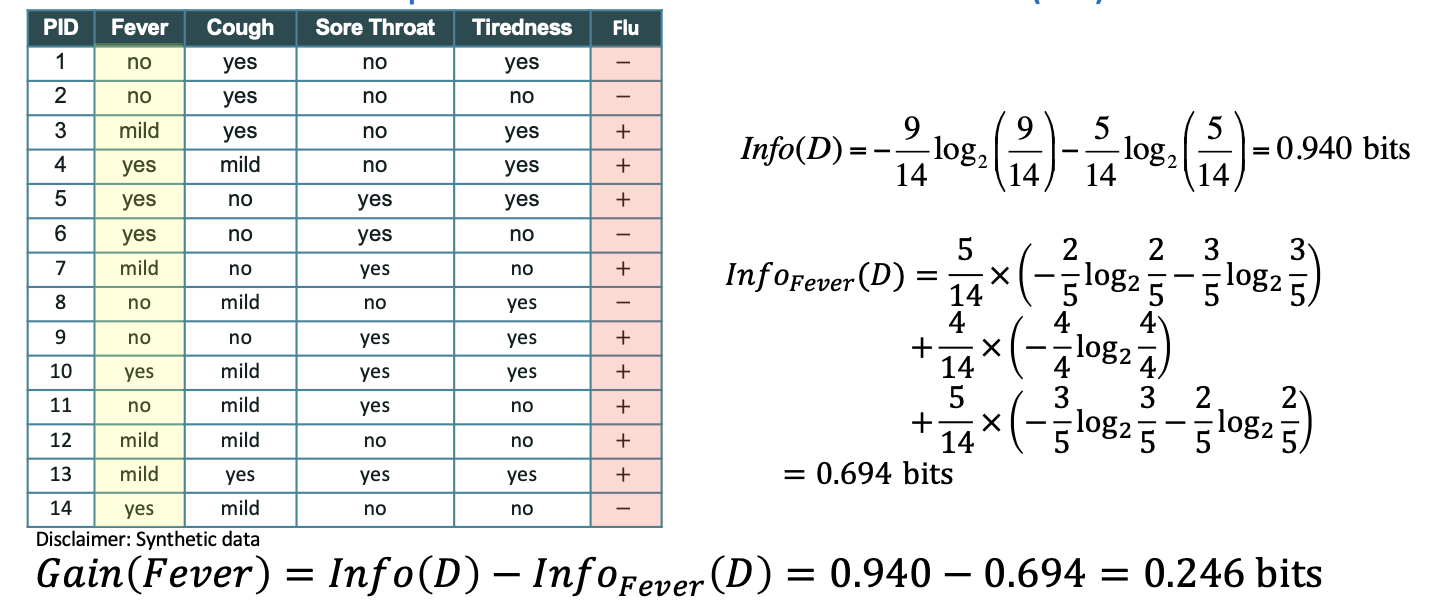
\includegraphics[scale=0.36]{images/Information_Gain.png}

\quad

$SplitInfo_A(D) = -\sum_{j=1}^{v} \frac{|D_j|}{|D|} \log_2\left(\frac{|D_j|}{|D|}\right)$

$GainRatio_A(D) = \frac{\text{Gain}(A)}{\text{SplitInfo}_A(D)}$

\bulletPoint{Gini Index}:

$\text{Gini}(D) = 1 - \sum_{i=1}^{2} p_i^2 \quad \text{Gini}_A(D) = \frac{|D_1|}{|D|} \text{Gini}(D_1) + \frac{|D_2|}{|D|} \text{Gini}(D_2)$

$\Delta \text{Gini}(A) = \text{Gini}(D) - \text{Gini}_A(D)$

\bulletPoint{Evaluating Classifier Performance}:

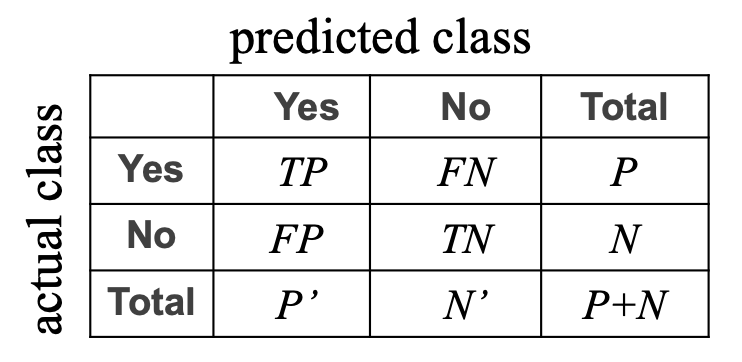
\includegraphics[scale=0.4]{images/TP.png}

$\text{Accuracy} = \frac{TP + TN}{P + N} \quad  \text{Error rate} = \frac{FP + FN}{P + N} = 1 - \text{Accuracy}

$ \text{Sensitivity} = \frac{TP}{P} \quad \text{Specificity} = \frac{TN}{N} $

$ \text{Accuracy} = \text{Sensitivity} \times \left(\frac{P}{P+N}\right) + \text{Specificity} \times \left(\frac{N}{P+N}\right) $

$ \text{Precision} = \frac{TP}{TP + FP} = \frac{TP}{P'} $ 

$\text{Recall} = \frac{TP}{TP + FN} = \frac{TP}{P} = TPR \quad \frac{FP}{N} =FPR $

$ F = \frac{2 \times \text{Precision} \times \text{Recall}}{\text{Precision} + \text{Recall}} $

%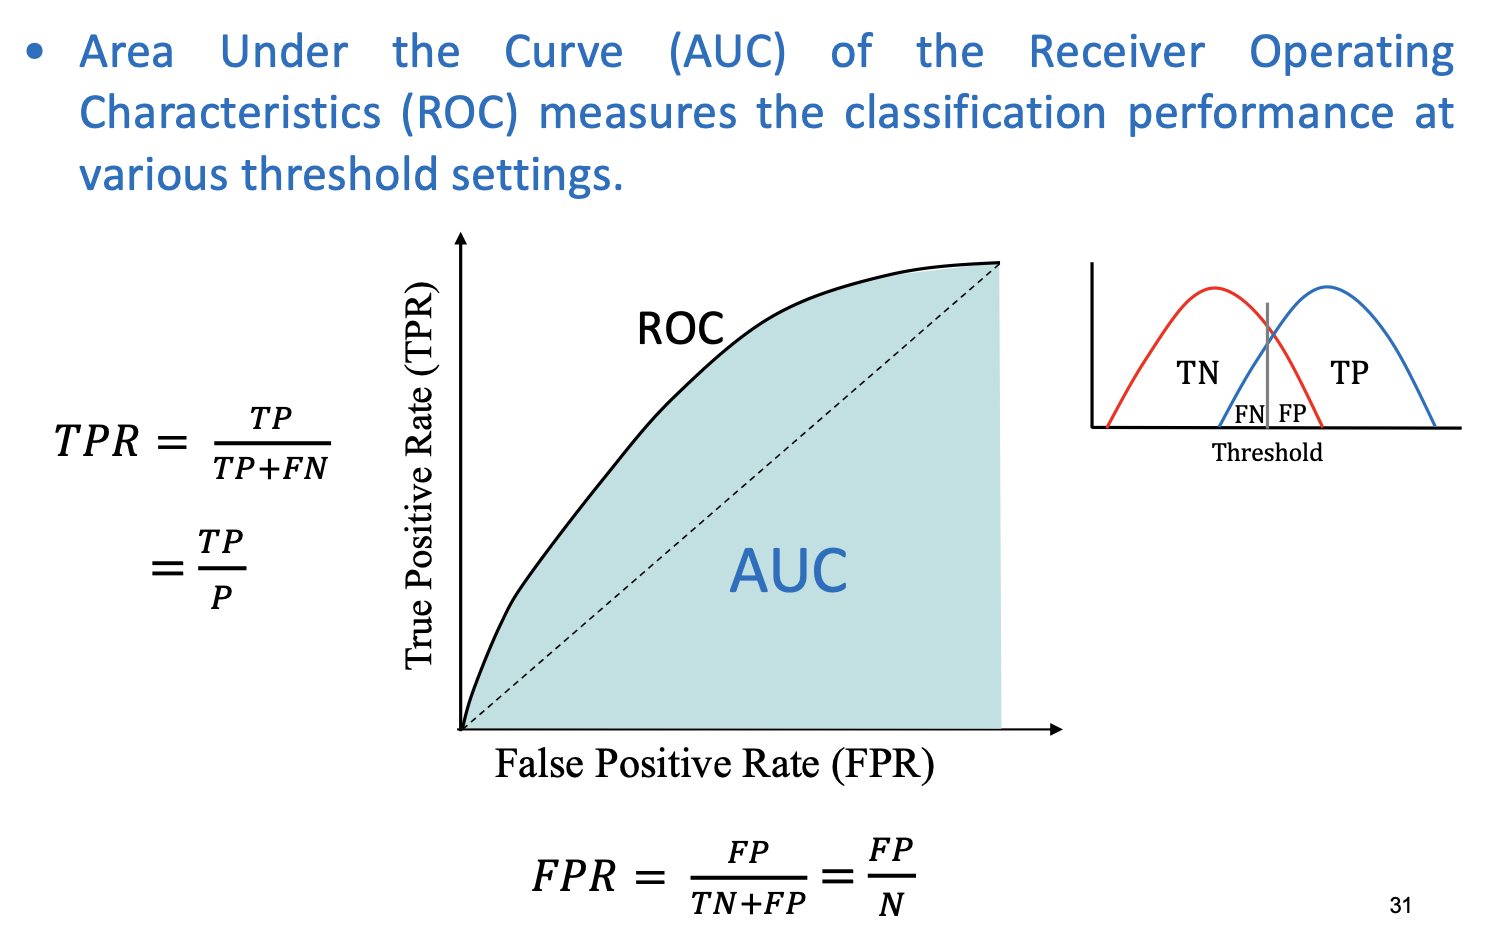
\includegraphics[scale=0.25]{AUC.png}

\bulletPoint{Dissimilarity and Similarity Measures}:

1. Minkowski distance:
$d(\mathbf{x}, \mathbf{y}) = \left( \sum_{k=1}^n |x_k - y_k|^r \right)^{1/r}$

2. Manhattan distance ($r = 1$):
$d(\mathbf{x}, \mathbf{y}) = \sum_{k=1}^n |x_k - y_k|$

3. Euclidean distance ($r = 2$):
$d(\mathbf{x}, \mathbf{y}) = \sqrt{\sum_{k=1}^n (x_k - y_k)^2}$

4. Cosine similarity:
$ \cos(\mathbf{x}, \mathbf{y}) = \frac{\mathbf{x} \cdot \mathbf{y}}{\|\mathbf{x}\| \|\mathbf{y}\|} = \frac{\sum_{i=1}^n x_i y_i}{\sqrt{\sum_{i=1}^n x_i^2} \sqrt{\sum_{i=1}^n y_i^2}}$

5. Infinity (Sup) Distance: 
$ d(\mathbf{x}, \mathbf{y}) = \max_{1 \leq j \leq d} |x_j - y_j| $

\bulletPoint{SVM}:

$ y_i = \text{sign}(\mathbf{w} \cdot \mathbf{x}_i + b). \quad d = \frac{2}{\|\mathbf{w}\|}. $

$ \min_{\mathbf{w}} \frac{\|\mathbf{w}\|^2}{2} \quad \text{subject to} \quad y_i(\mathbf{w} \cdot \mathbf{x}_i + b) \geq 1, \; i = 1, 2, \dots, N. $

–  Dual optimization problem

$ \mathbf{w} = \sum_{i=1}^N \lambda_i y_i \mathbf{x}_i, \quad \sum_{i=1}^N \lambda_i y_i = 0. $

$ y_i(\mathbf{w} \cdot \mathbf{x}_i + b) - 1 = 0. $


\bulletPoint{Neural Network}:

– Activation Functions:

Linear: $ \sigma(x) = x \quad$
Sigmoid: $ \sigma(x) = \frac{1}{1 + e^{-ax}} $ \quad Tanh: $ \sigma(x) = \tanh(\gamma x) = \frac{e^{2\gamma x} - 1}{e^{2\gamma x} + 1} $

Sign: $ \sigma(x) = \text{sign}(x) = 
\begin{cases} 
+1, & x \geq 0 \\
-1, & x < 0 
\end{cases} $ \quad ReLU: $ \sigma(x) = 
\begin{cases} 
x, & x \geq 0 \\
0, & x < 0 
\end{cases} = \max(0, x) $

Leaky ReLU: $ \sigma(x) = 
\begin{cases} 
x, & x \geq 0 \\
ax, & x < 0 
\end{cases} = \max(ax, x), \quad \text{where } a \ll 1 $

– Gradient Descent: 
$ \mathbf{w}' = \mathbf{w} - \eta \frac{\partial J(\mathbf{w})}{\partial \mathbf{w}} $

– Back propagation Algorithm:

% $ E = \frac{1}{2} \sum_{k=1}^c (t_k - o_k)^2 = \frac{1}{2} \| \mathbf{t} - \mathbf{o} \|^2 \quad
% \Delta w_{jk} = -\eta_w \frac{\partial E}{\partial w_{jk}} \quad
% \Delta b_j = -\eta_b \frac{\partial E}{\partial b_j} $

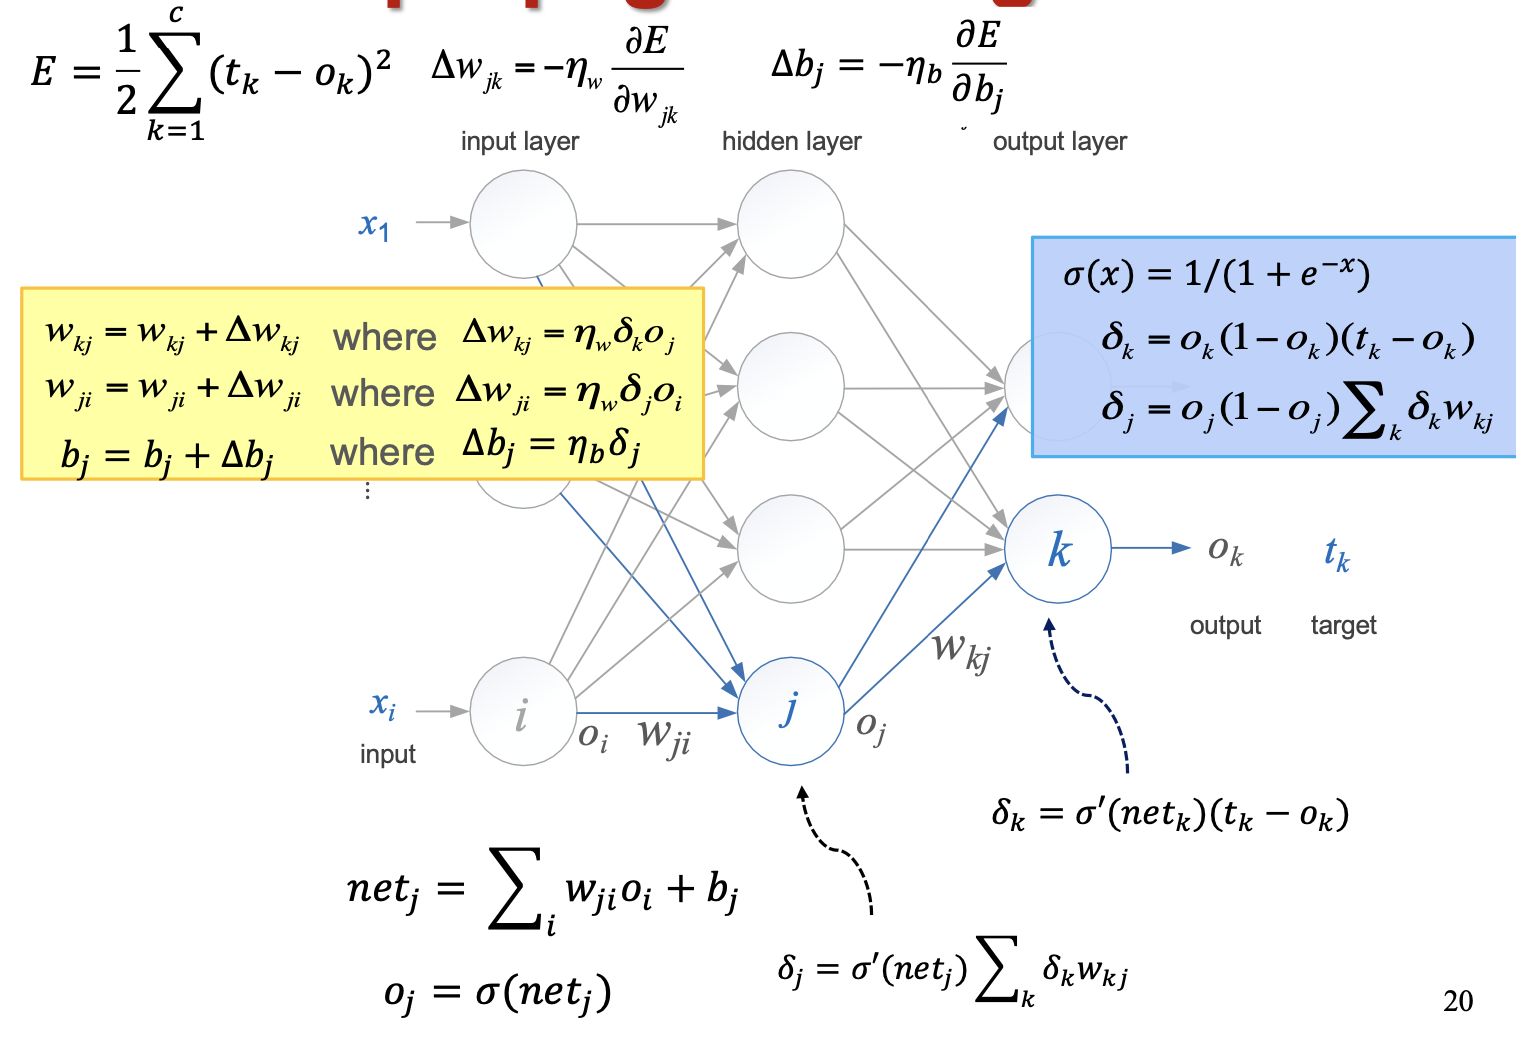
\includegraphics[scale=0.38]{images/NN.png}

% $ w_{kj} = w_{kj} + \Delta w_{kj}, \quad \text{where} \quad \Delta w_{kj} = \eta_w \delta_k o_j $

% $ w_{ji} = w_{ji} + \Delta w_{ji}, \quad \text{where} \quad \Delta w_{ji} = \eta_w \delta_j o_i $

% $ b_j = b_j + \Delta b_j, \quad \text{where} \quad \Delta b_j = \eta_b \delta_j $

% $\text{net}_j = \sum_i w_{ji} o_i + b_j \quad o_j = \sigma(\text{net}_j) $

$ \delta_k = \sigma'(\text{net}_k)(t_k - o_k), \quad \text{for output units} $

$ \delta_j = \sigma'(\text{net}_j) \sum_k \delta_k w_{kj}, \quad \text{for hidden units} $

\quad

$
\frac{\partial E}{\partial w_{kj}} = \frac{\partial E}{\partial o_k} \cdot \frac{\partial o_k}{\partial \text{net}_k} \cdot \frac{\partial \text{net}_k}{\partial w_{kj}}  
= \frac{\partial E}{\partial o_k} \cdot \sigma'(\text{net}_k) \cdot \frac{\partial (\sum_j w_{kj} o_j + b_k)}{\partial w_{kj}}  
= -(t_k - o_k) \cdot \sigma'(\text{net}_k) \cdot o_j 
= -\delta_k \cdot o_j
$

$ \frac{\partial E}{\partial w_{ji}} = \frac{\partial E}{\partial o_j} \cdot \frac{\partial o_j}{\partial \text{net}_j} \cdot \frac{\partial \text{net}_j}{\partial w_{ji}} 
= \frac{\partial E}{\partial o_j} \cdot \sigma'(\text{net}_j) \cdot \frac{\partial \left(\sum_i w_{ji} o_i + b_j\right)}{\partial w_{ji}} 
= -\left(\sum_k \delta_k w_{kj}\right) \cdot \sigma'(\text{net}_j) \cdot o_i 
= -\delta_j \cdot o_i $

\bulletPoint{CNN}:

– Stride: steps per moving.  – Zero padding : pads the input with zeros around the border.   – Pooling: Max: max one within filter size; Average: average within filter size. 

– Regularization: $ J'(\mathbf{w}) = J(\mathbf{w}) + \alpha R(\mathbf{w}) $

L1 Regularization (LASSO): $ R(\mathbf{w}) = \|\mathbf{w}\|_1 = \sum_k |w_k| $

L2 Regularization (Ridge): $ R(\mathbf{w}) = \|\mathbf{w}\|_2^2 = \sum_k (w_k)^2 $

Elastic Net Regularization: $ R(\mathbf{w}) = \|\mathbf{w}\|_1 + \beta \|\mathbf{w}\|_2^2 $

Also can be done by early stopping. 

\bulletPoint{Clustering}:

– Use Euclidean Distance: $d(\mathbf{x}, \mathbf{y}) = \sqrt{\sum_{k=1}^n (x_k - y_k)^2}$

– K-Means: 1. Initialize K random points as K clusters' centers. 2. Assign every point to its cluster by which center it nearest. 3. Calculate each clusters' average again to set as new center. 4. Repeat 2-3, until no points assignments.    Initialization influence results. 

– HAC: 
--Single Linkage: the minimum distance between any pair of two data samples from each cluster. 
 --Complete Linkage: the maximum distance between any pair of two data samples from each cluster. 
 --Average Linkage: the average distance between all pairs of two data samples from each cluster.    
 --Centroid Distance: the distance between the means of data samples (i.e., centroids) from each cluster.

• What is the limitations of K-Means algorithm?
Need to choose K. Can stuck at poor local minimum. Need good metric.
• What are the limitations of HAC algorithm?
Memory- and computationally-intensive.

\bulletPoint{Regression}:

$ f_{w,b}(\mathbf{x}) = \mathbf{w}^T \mathbf{x} + b $

Minimize the \( l_2 \) loss: $ \min_{\mathbf{w}, b} \hat{L}(f_{w,b}) = \min_{\mathbf{w}, b} \frac{1}{N} \sum_{i=1}^N \left( \mathbf{w}^T \mathbf{x}_i + b - y_i \right)^2 $

$ \text{Loss function: mean squared error between } \mathbf{w}^T \mathbf{x}_i + b \text{ and } y_i. $


\bulletPoint{Bias and Variance}:

– Bias: Error caused by the wrong assumptions made in the learning algorithms or models.

– Variance: Error due to the learning sensitivity to small fluctuations in the training set.

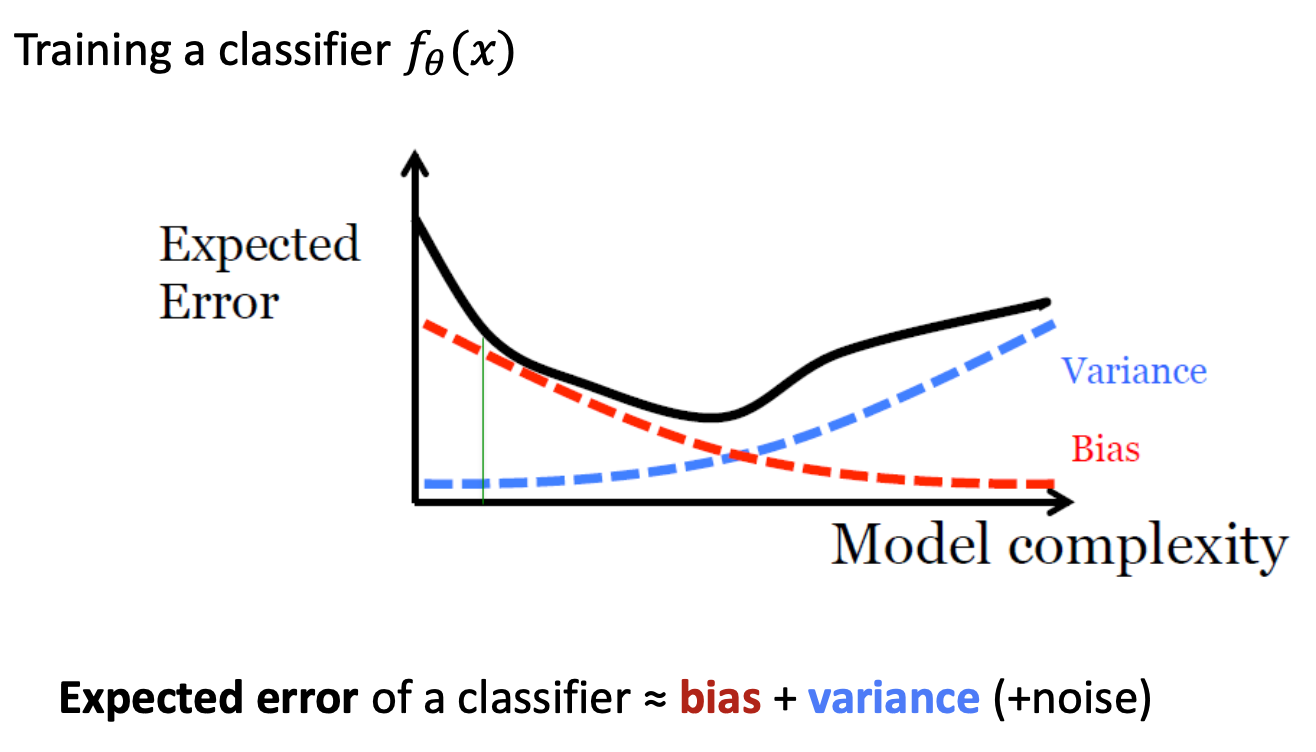
\includegraphics[scale=0.27]{images/bias & variance.png}

– Underfitting: High bias and low variance. 

– Overfitting: Low bias and high variance. 

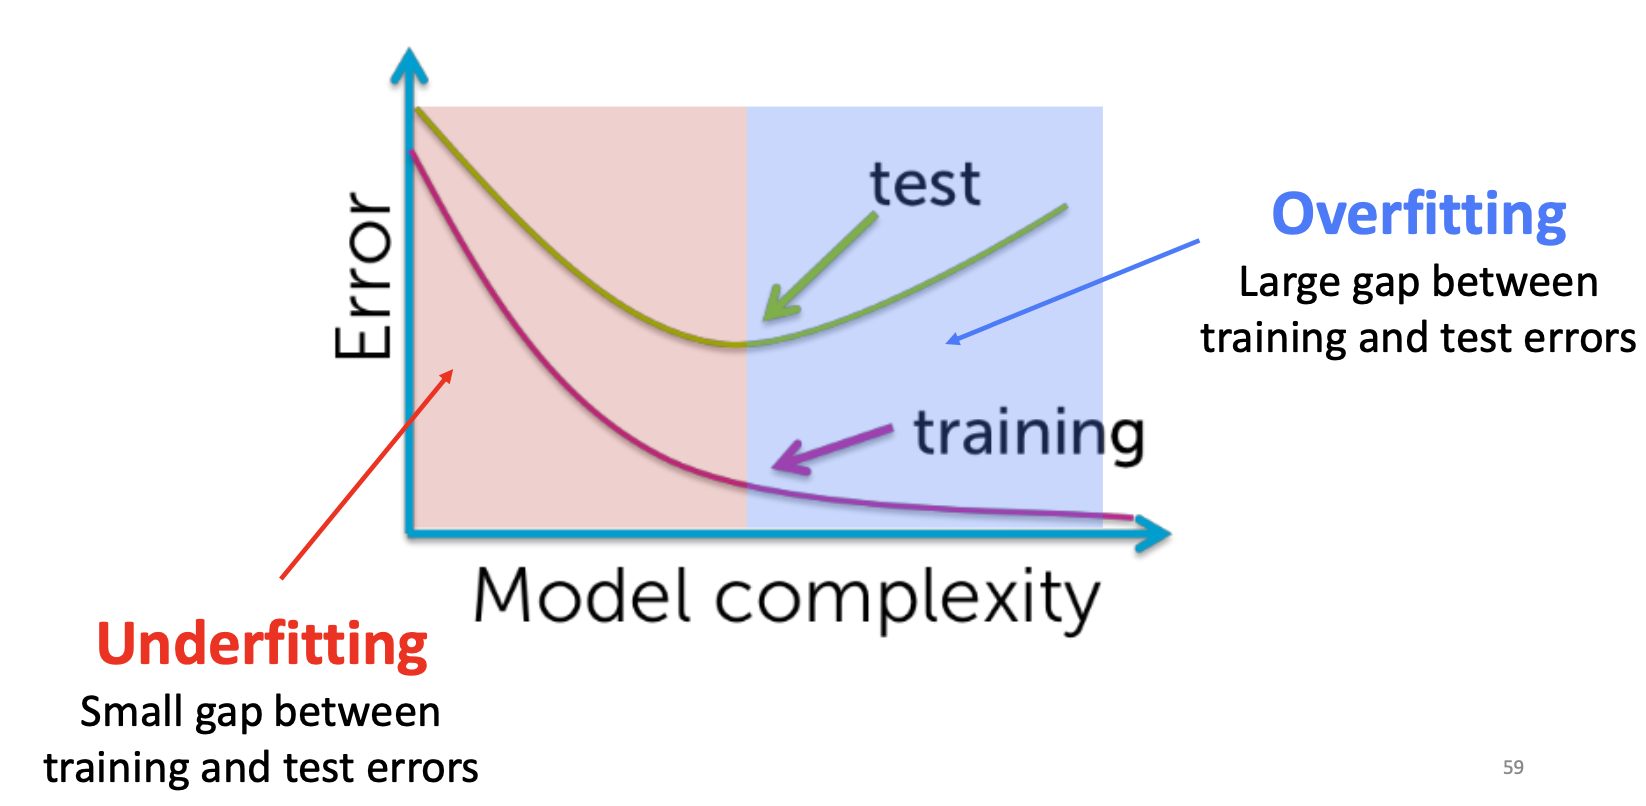
\includegraphics[scale=0.235]{images/over-under-fitting.png}


\bulletPoint{PCA}:

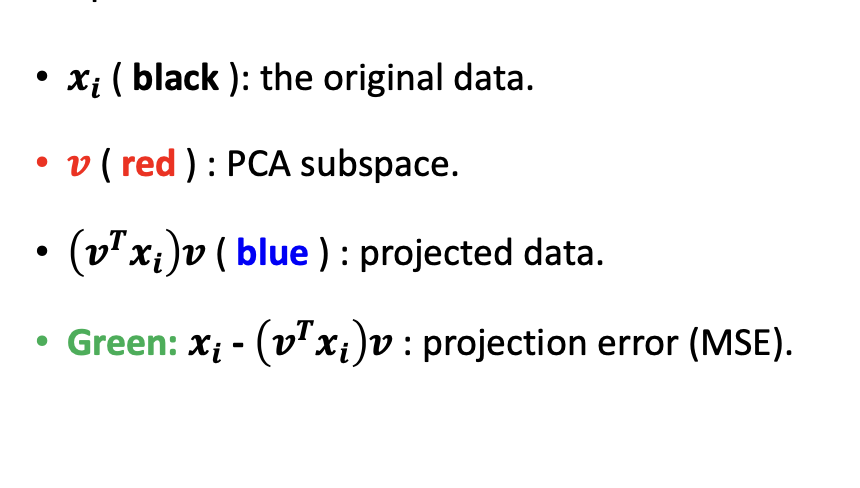
\includegraphics[scale=0.35]{images/PCA1.png}
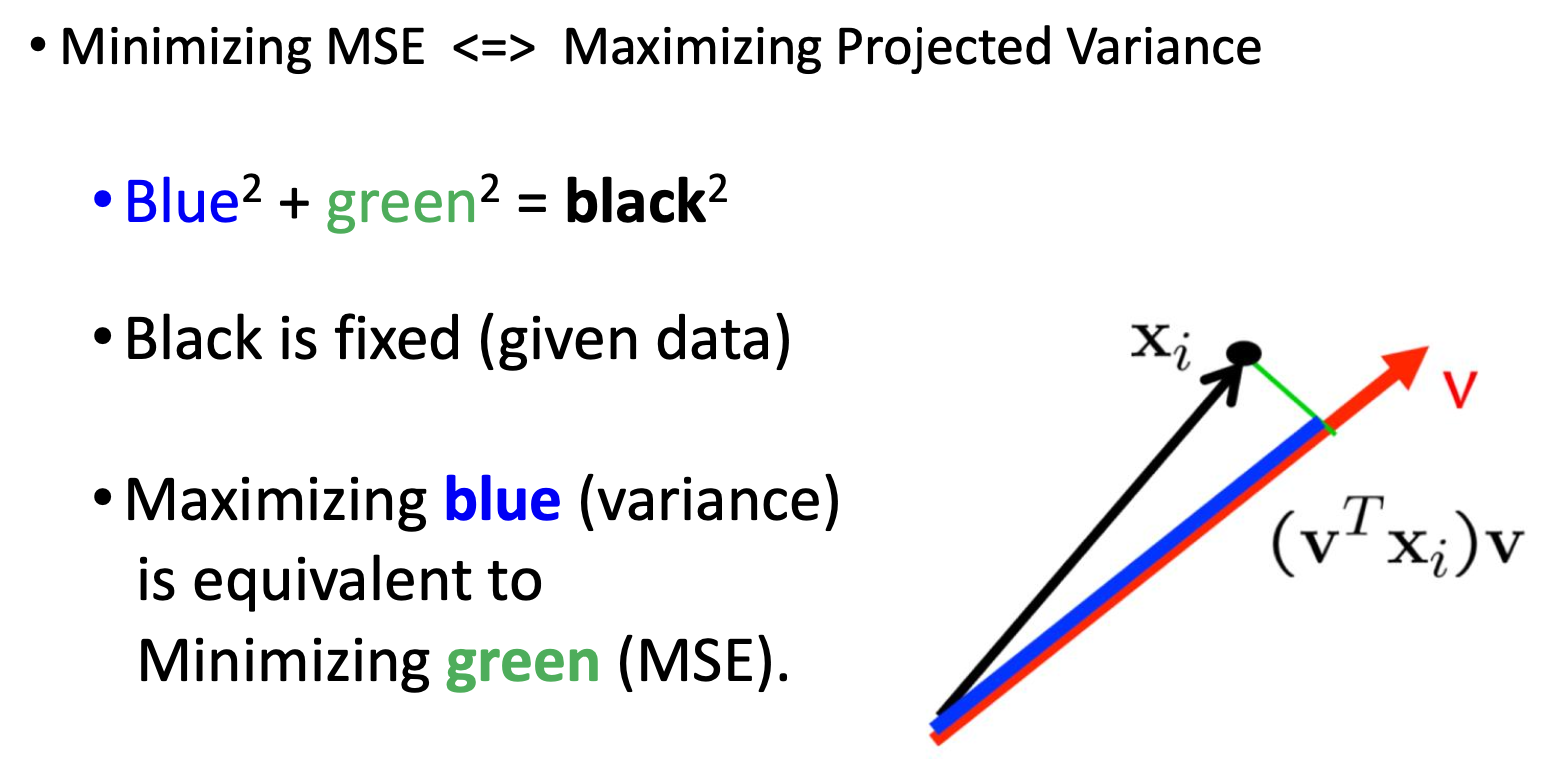
\includegraphics[scale=0.26]{images/PCA2.png}


\bulletPoint{Bayes’ Theorem}:

$ P(A \mid B) = \frac{P(B \mid A) P(A)}{P(B)}  $

$ P(B) = \sum_i P(B \mid A_i) P(A_i) $

\bulletPoint{Naïve Bayes}:

$ P(a_1, \dots, a_d \mid v_j) = P(a_1 \mid v_j) \cdots P(a_d \mid v_j)  = \prod_{i=1}^d P(a_i \mid v_j) $


\end{multicols*}

\end{document}